\documentclass[a4paper, oneside, 10pt]{book}

\usepackage{fancyhdr,verbatim, listings, color} 
\usepackage{shorttoc}
\usepackage[english]{minitoc}
\usepackage[pdftex]{graphicx} 
\usepackage[utf8]{inputenc}
\usepackage[T1]{fontenc}
\usepackage[english]{babel}
\usepackage{amsmath,amssymb,mathrsfs}
\usepackage[english]{varioref}
\usepackage{url}
\usepackage{../nota}
\usepackage{../citation}
%\usepackage{../sommaire}

\graphicspath{%
  {../imgs/}%
  {imgs/}
}

% NOTES
\setlength{\largeurnota}{.8cm}
\newenvironment{attention}{%
  \begin{pictonote}{attention}}{\end{pictonote}}
\newenvironment{note}{%
  \begin{pictonote}{note}}{\end{pictonote}}
\newenvironment{question}{%
  \begin{pictonote}{question}}{\end{pictonote}}

\usepackage[pdftex=true,
    bookmarks         = true,
    bookmarksnumbered = true,
    bookmarks = true, 
    pdfstartview      = FitH,
    bookmarksopen     = true, 
    bookmarksopenlevel = 1, 
    hyperindex        = true,
    colorlinks        = true,
    %urlcolor          = red,
    %pdfborder         = {0 0 0}
    ]{hyperref}

\definecolor{colKeys}{rgb}{0,0,1} 
\definecolor{colIdentifier}{rgb}{0,0,0} 
\definecolor{colComments}{rgb}{0,0.5,1} 
\definecolor{colString}{rgb}{0.6,0.1,0.1} 

\lstset{
float=hbp,
basicstyle=\ttfamily\small,
identifierstyle=\color{colIdentifier},
keywordstyle=\color{colKeys},
stringstyle=\color{colString},
commentstyle=\color{colComments},
language=c++,
columns=flexible,
tabsize=2,
frame=trBL,
frameround=tttt,
extendedchars=true,
showspaces=false,
showstringspaces=false,
numbers=left,
numberstyle=\tiny,
breaklines=true,
breakautoindent=true,
captionpos=b,
commentstyle=\textit
}

\lstnewenvironment{cpp}{\lstset{language=c++}}{}

%% Define a new 'leo' style for the package that will use a smaller font.
\makeatletter
\def\url@leostyle{%
  \@ifundefined{selectfont}{\def\UrlFont{\sf}}{\def\UrlFont{\small\ttfamily}}}
\makeatother
%% Now actually use the newly defined style.
\urlstyle{leo}

\pagestyle{fancy} 



\hypersetup{
    pdfauthor   = {Arnaud Audoin, Clément Badiola, Samuel Da Silva, Alexandre Perrot, Camille Ritlewski},% 
    pdftitle    = {PER - Rapport final},%
    pdfsubject  = {Rapport final},% 
    pdfkeywords = {},% 
    pdfcreator  = {PDFLaTeX},% 
    pdfproducer = {PDFLaTeX}} 

\author{Arnaud~\textsc{Audoin} \and Clément~\textsc{Badiola} \and Samuel~\textsc{Da~Silva} \and Alexandre~\textsc{Perrot} \and Camille~\textsc{Ritlewski} \and \\
  Client : Paul~\textsc{Dorbec}}
\title{The map coloring game \\ Final report}
\date{24 janvier 2013}

\begin{document}

\graphicspath{{../imgs/}}

\fancyhf{} 
\renewcommand{\chaptermark}[1]{\markboth{#1}{}} 
\renewcommand{\sectionmark}[1]{\markright{\thesection\ #1}} 
\fancyhead[R]{\bfseries\thepage}% Left Even, Right Odd - No de page 
\fancyhead[L]{\bfseries\rightmark} % Left Odd - Titre section 
\renewcommand{\headrulewidth}{0.5pt}% filet en haut de page 
\addtolength{\headheight}{0.5pt} % espace pour le filet 
\renewcommand{\footrulewidth}{0pt} % pas de filet en bas 
\fancypagestyle{plain}{ % pages de tetes de chapitre 
  \fancyhead{} % supprime l’entete 
  \renewcommand{\headrulewidth}{0pt} % et le filet 
}

\fancypagestyle{plain}{
	\fancyhf{}
	\fancyfoot[C]{\thepage}
	\renewcommand{\headrulewidth}{0pt}
	\renewcommand{\footrulewidth}{0pt}}

\dominitoc

\maketitle

\frontmatter

%pour moi, on ne peut pas exposer le problème avant d'avoir fait l'introduction et expliqué le domaine…. 
%\section*{Abstract}
This document is the final report of a research project carried out by a group of 5 students within their year of Master 2.

The project addresses the graph coloring game, a variant of the graph coloring problem, by using Monte Carlo heuristics and statistical tools to determine whether the theoretical bounds calculated by the researchers can be improved.

The results, presented in detail later, suggest that the current theoretical bounds can be significantly improved. %Enoncé du problème et des objectifs puis résumé (synthèse d'une page max.) du projet

\tableofcontents

\mainmatter

\chapter{Introduction}

\section{Graph coloring}

Graph coloring is not a new problem in mathematics and computer science. The first results in this field date back to 1852, when \emph{Francis Guthrie} postulated the famous four color theorem\footnote{He did not write any publication on this theorem.}.

Coloring a graph consists in assigning a color to each vertex of the graph, so that two adjacent vertices are of different colors. Such a coloring is called a proper coloring. There are other forms of coloring, such as edge or face coloring, but they always amount to a vertex coloring on another graph.

A graph is said to be k-coloriable if it admits a proper coloring with k colors. The minimal number of colors needed to achieve a proper coloring of a particular graph is called the \textit{chromatic number} of that graph, noted $ \chi (g)$. Deciding if a graph is k-coloriable for a given value of k is NP-complete.

\section{Map-coloring game}

The studied article's subject defines a variant of the graph coloring involving two players.

The first player tries to color the graph correctly. The second tries to hinder and stop him without overriding the coloring rule. The coloring rule stays the same: each vertex cannot have the same color as its neighbors. 
At the beginning of the game, we set a number N of colors than can be used in the game. The game ends if all the vertices are colored or if it is not possible to color the graph without adding a color while exceeding N, which is contrary to the rules.

 
We defines the \textit{game chromatic number} as the minimal number of colors with which the first player can achieve a correct coloring of the graph whatever the strategy of the second player.

\section{Exemple of a game}

%\begin{figure}[h]
%\begin{center}
%    \includegraphics[width=11cm]{nom-du-fichier-image}
%\end{center}
%    \caption{phrase de legende pour limage}
%    \label{nom de la reference latex vers limage si on veut la citer dans le texte}
%\end{figure}
\section{Applications}

The graph coloring game has no direct applications. It helps to get a better understanding of the field of graph coloring.

Graph coloring applications examples:
\begin{itemize}
\item memory allocation,
\item management of a room's occupation, 
\item management of schedules etc.
\end{itemize}





%\vfill
%
%\textbf{Mots-clés :} mot clef 1, mot clef 2, macFly
%
%\vfill
 %Définir le probleme, les objectifs, le cadre de travail (contexte).


%l'état de l'art se trouve dans l'introduction
%\chapter{Documentation}
\minitoc

%\section{Historique}
\section{Historique}

\begin{description}
\item[1940] Invention de la loupe téléscopique.
\item[1943] McFly et Marty inventent la voiture à remonter le temps. 
\end{description}

Depuis, les recherches sur les sulfatrons pulsatifs ionisés n'ont cessé d'amener de nouvelles applications, en combinant parfois plusieurs modèles.




%\section{Modèles courants}
\section{Modèles courants}


%\section{Utilisations}
\section{Utilisations}

De part leur fort potentiel pour résoudre des problèmes de nature biotroniques, les produits lactiques représentent un secteur de recherche très attractif pour les PME. Voilà.



 %etat de l'art (contexte technique et scientifique), bibliographie importante.

%%%%%% Stratégies tirées de l'article
\chapter{Théorie}

 %théorie spécifique à notre probleme (les differents théoremes) (les détails seront a mettre en annexe).

\chapter{Work}
\minitoc

\section{Monte Carlo}

Monte-Carlo methods are a set of randomized algorithms. The general idea is to use random samplings rather than computing to help solve a problem. Such algorithms are mostly used when computing a solution to the problem is not feasible. Because of the use of random samplings, these are heuristics by nature : their results are not always guaranteed to be exact. Throughout the years, Monte-Carlo methods have been successfully used in physics, mathematics  and computer sciences.\\


In this report, we will interest ourselves in a special case of Monte-Carlo methods : Monte-Carlo tree search, aka MCTS. It applies Monte-Carlo principles to trees exploration. The main field of application is artificial intelligence, especially games with very large move space where a complete tree exploration is not possible in reasonable time, such as Chess and Go.\\

MCTS is composed of four steps : selection, expansion, simulation and backpropagation. Those steps are repeated until time runs out, the maximum number of simulated games has been played, a satisfying result is found or whatever condition is relevant. Generally, the more iterations are run, the more accurate is the result.

The selection step chooses a node in order to play a simulation from it. Several algorithms exist for this stage, depending on the context. The expansion step produces childs of the selected node if not already generated. This step makes the search tree grow in height. The simulation step plays the game until the end following nodes selected with a selection algorithm which can be the same as the one used in the selection step or a different one. Finally, th backpropagation step uses the outcome of the simulated game to modify the estimated value of the traversed nodes. This is the crucial step to know what has been played and if the selected moves constitute good choices or not.

After playing enough simulated games, a player can then choose amongst the playable moves which one to play using the estimated value of the move. The choice algorithm can be one of the followings (from \cite{ChaPHD}) :
\begin{itemize}
\item Max Child : Choosing the node with the highest value.
\item Robust Child : Choosing the node with the highest number of games played.
\item Robust-Max Child : Choosing the node with both the best value and highest number of games played.
\item Secure Child : Choosing the node maximizing a lower confidence bound.\\
\end{itemize}


\begin{figure}
\centering
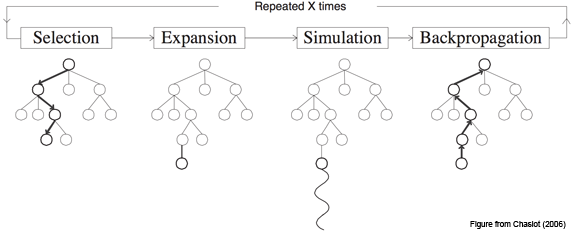
\includegraphics[width=11cm]{mcts-algorithm.png}
\caption{Etapes de Monte-Carlo tree search}
\label{treesearch}
\end{figure}

According to \emph{Guillaume Chaslot} \cite{ChaPHD} : "MCTS is
applicable if at least the following three conditions are satisfied: (1) the payoffs are bounded
(the game scores are bounded), (2) the rules are known (complete information), and (3) simulations terminate relatively fast (game length is limited)". Those three criterias are verified in the case of the map-coloring game. We will use Monte-Carlo tree search to implement an AI capable of playing Alice or Bob.\\

\section{How our AI works}

To modelise a map-coloring game, each node of the exploration tree will contain:
\begin{itemize}
\item The move played when choosing that node, which is simply the node chosen in the game graph and the color used.
\item The total number of games played through that node.
\item The number of games with a favorable outcome for Alice while playing through that node.
\end{itemize}
For each node in the search tree, its value can be seen as the victory ratio for Alice : (games won/games played).\\

The selection algorithm we used is based on multi-armed bandit algorithms as described in \cite{MAB}. Indeed, selecting a node amongst the children of the current node in the tree can be seen as a multi-armed bandit problem, where each node is a bandit, its profit being its value. We chose the UCT algorithm, based on the UCB1 multi-armed bandit algorithm, described in \cite{ChaPHD}. This algorithm is called best-first because it always selects the node which seems to be the best. This estimation is based on the value of the node and an upper confidence bound. This bound only depends on the number of games played in the node and its parent. For every game played through a node, the upper confidence bound of this node is reduced. This is a formal way of describing an intuitive idea : "The more I play this move, the more I am confident in the value I have calculated". The best node according to the algorithm is the node whose value plus upper confidence bound is the highest. By using this algorithm, we can quickly stop exploring the least interesting nodes to concentrate on better ones, thus maximizing the profit from a fixed number of simulations.\\

%Introduction du terme zero-sum : pas expliqué, explication nécessaire donc (footnote par exemple ?)
Nevertheless, this algorithm is adapted to a general Monte-Carlo tree search. In our particular case, we deal with a game between two opponents whose objectives are opposite. Using this algorithm directly would bring us to consider that the opponent is playing toward the same goal, thus helping us, which is of course false. The canonic way of dealing with that problem in a two-player zero-sum game is called Minimax (established in \cite{Minimax}). When exploring a tree with Minimax, the values are maximized when playing with player 1 and minimized when playing player 2, to represent the opposite goal. We reproduced a similar process in the UCT algorithm. If Alice is playing, the confidence interval of the node is added to its value, and the chosen node is the one with the highest resulting total. On the contrary, if Bob is playing, the confidence interval is substracted from the value, resulting in a lower confidence bound. The selected node is then the one with the lowest lower confidence bound.
Using this minimax UCT algorithm, our AI implementation will be the same both for Alice and Bob.\\

The other steps of the Monte-Carlo tree search are now straightforward. The expansion step just generates every legal move on the graph from the current position with the currently used colors, and moves with a new colors and adds a node for each one. The simulation step reuses the selection algorithm to play until the game is finished. Finally, the backpropagating step increments the number of games played and won according to the outcome of the game.\\

%Dans Monte Carlo, on va chercher à jouer beaucoup de parties pour un graph donné (que nous appellerons le graph étudié) afin de pouvoir jouer les meilleurs coups possibles. 
%Pour chaque graph étudié, nous générons un arbre des coups joués où chaque nœuds, sauf la racine, correspondent à des coups joués sur ce graph. 
%
%Ce que contient un nœud de l’arbre généré : 
%\begin{itemize}
%\item le nœud joué dans le graph étudié
%\item la couleur jouée sur ce nœud 
%\item le nombre de partie jouées en passant par ce nœud 
%\item le nombre de partie gagné par Alice en passant par ce nœud
%\end{itemize}
%
%Au début l’arbre ne contient que la racine et les premiers coups possibles. Nous n’avons aucune connaissance des coups qui amènent à colorier proprement le graph étudié ni de ceux qui nous mettrons  dans une situation bloquante. 
%
%Afin de limiter le nombre de fils, nous allons éliminé des coups équivalents : nous considérons que les couleurs sont numérotées et qu’il est impossible de jouer une couleur n, si la couleur n-1 n’a pas encore été jouée. En effet il est équivalent d’introduire la couleur n-1 ou la couleur n. 
%
%D’autre part nous allons généré le graph au fur et a mesure des parties et des coups joués. À chaque fois que l’on est dans un nœud (i.e. on viens de jouer le coup correspondant dans le graph étudié), si il n’a pas de fils, on regarde l'état de la partie : 
%\begin{itemize}
%\item soit la partie est finie (Alice a gagné ou Bob à gagné), on remonte alors jusqu’à la racine en mettant à jour tous les nœuds sur le chemin. Si Alice a gagné (i.e. le graph étudié est entièrement colorié) on incrémente le nombre de partie joué et le nombre de partie gagné. Si Alice n’a pas gagné (i.e. le graph étudié n’est pas entièrement colorié)  on incrémente juste le nombre de partie joué.
%\item soit on peut continuer (auquel cas on génère les fils et on continue la simulation récursivement).
%\end{itemize}
%Quand on a joué dans un nœud, on a un pourcentage de victoire pour le coup correspondant, mais il n’est pas forcément représentatif. Le fait de jouer plus de parties va permettre de diminuer l'intervalle de confiance de ce ratio de victoire.
%
%%\subsection {Algorithme de notre IA}
%Pour éviter de toujours passer par les mêmes nœuds, nous allons essayé passer par tous les frères d’un nœud déjà visité avant de pouvoir le revisiter pour explorer ces fils. Ce qui compte, ce sont surtout les coups au premier niveau (le niveau que l’on est en train d’étudier, les coups à jouer immédiatement). Les coups de niveau inférieur ne pourront pas être tous explorés, mais seront regardés de plus près quand on avancera dans le jeu et qu'ils arriveront au premier niveau.
%La partie délicate de Monte-Carlo est la sélection de nœud pour l'exploration. Dans un premier temps nous avons considéré  qu’il faut en priorité visiter le nœud qui a le moins de parties jouées, car il a été visité moins de fois que ses « frères ». Mais jouer celui le moins regardé pour l'instant n'est clairement pas la bonne solution sur le long terme. Il faut une solution adaptative, qui va jouer les coups moins regardés au début, puis qui va jouer les meilleurs pour vérifier que ce sont bien les meilleurs. Nous allons donc utiliser les algorithmes de Multi-armed bandit, plus particulièrement UCB1, qui donne de bons résultats.
%(ressource en anglais : \url{http://www.chrisstucchio.com/blog/2012/bandit_algorithms_vs_ab.html})
%(ressources en français : \url{http://researchers.lille.inria.fr/~munos/master-mva/lecture03.pdf}, \url{http://fr.slideshare.net/cornec/bandits-algo-klucb-par-garivier} )
%La seconde partie de Monte Carlo est l'exploitation. Une fois qu'on a effectué assez de simulations, on choisit un nœud pour le jouer "pour de vrai". Là encore, il y a plusieurs solution : on peut en effet prendre le nœud avec le meilleur ratio brut, mais on peut aussi prendre le nœud avec le meilleur ratio au mieux (plus l'intervalle de confiance) ou encore celui avec le meilleur ratio au pire (moins l'intervalle de confiance). 
%Sinon, pour la différence entre Alice et Bob, on se base sur une sélection min-max classique. Donc pour Alice on choisit le coup qui a le plus grand nombre de partie gagnée. Et pour Bob on choisit celui qui a le plus petit nombre de partie gagnée. 


\section{Implementation of the experiments}


In our program, many options are parametrizable. Those can be set using program arguments :
\begin{itemize}
\item The graph to play on (graphviz format supported)
\item The number of colors to play with
\item The number of games to play
\item The number of simulations to be run by Monte-Carlo before selecting a move
\end{itemize}
After some testing, we settled on the following experimental conditions :
\begin{itemize}
\item A number of simulations of 1000. This seemed to be a good compromize between speed and AI accuracy.
\item A number of games played of 1000. It seemed again to be a good compromize between computation time and statistical confidence. However, we could not play as much games on the 5x5 grids with a high number of colors (typically 4 or 5). We then tuned down the games to 100 for those cases. 
\end{itemize}

Here are the results :\\

\subsection{Chains}

\subsubsection{Odd number of vertices}

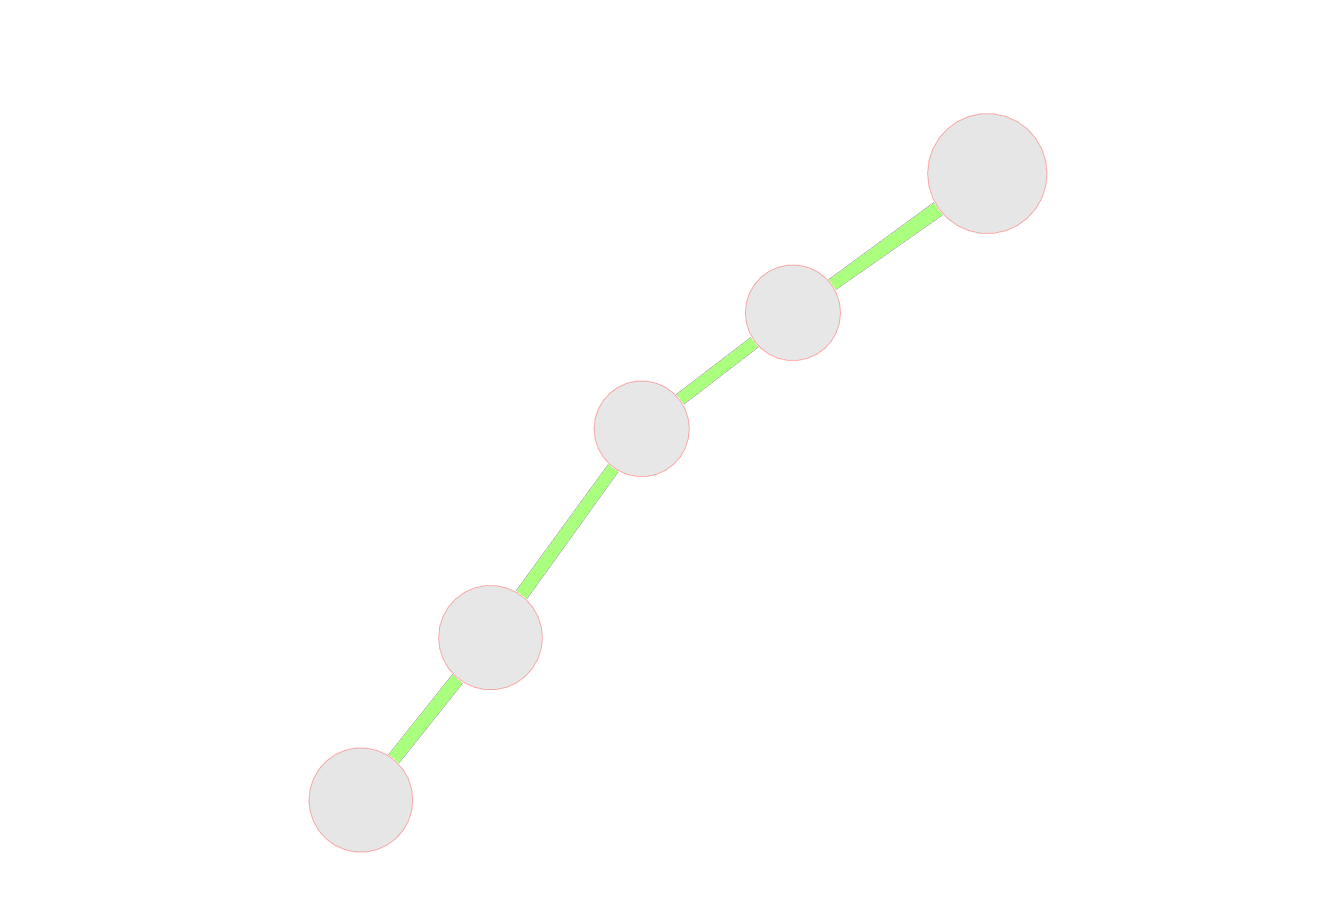
\includegraphics[width=11cm]{graphchaineimpaire.png}

\subsubsection{Even number of vertices}

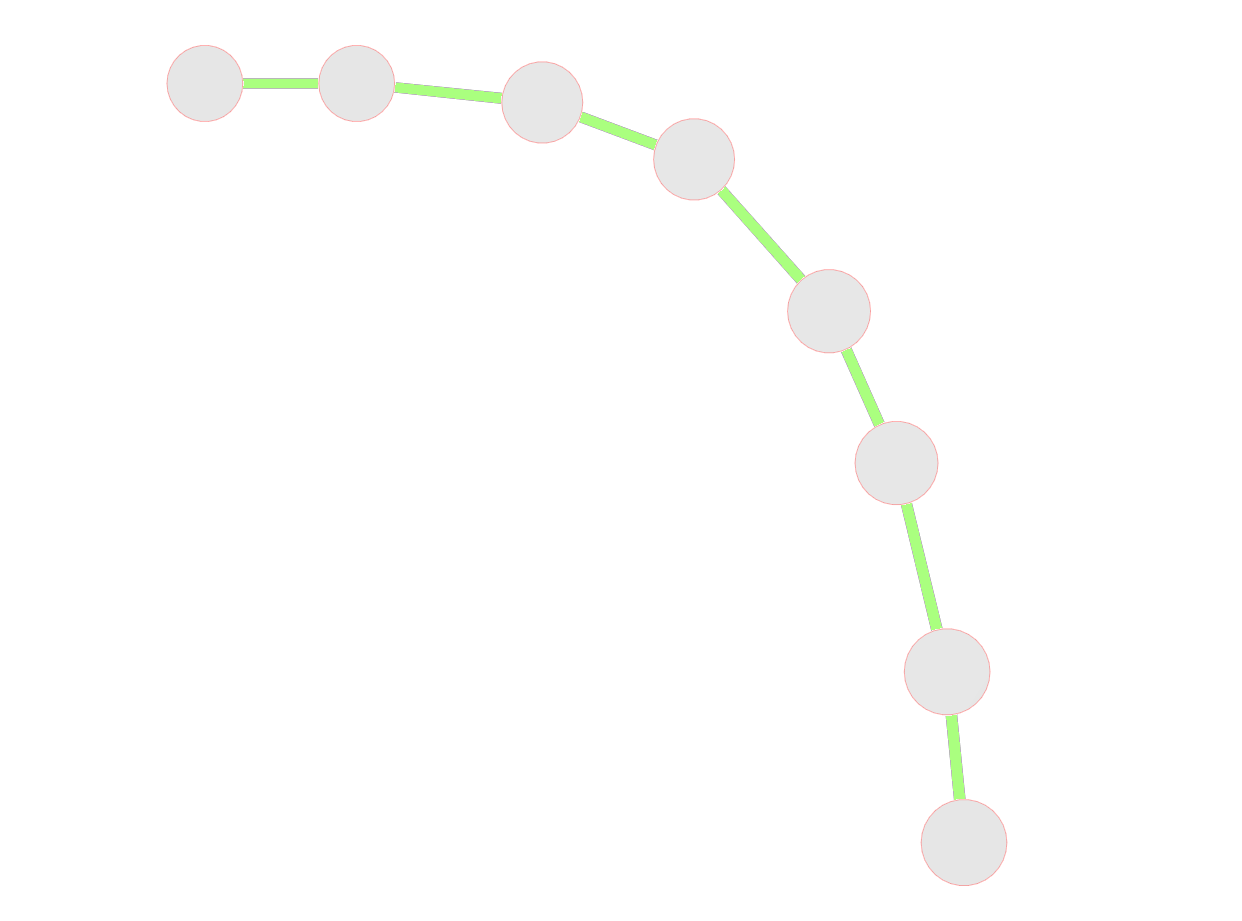
\includegraphics[width=11cm]{graphchainepaire.png}

\subsection{Cycles}

\subsubsection{Odd number of vertices}

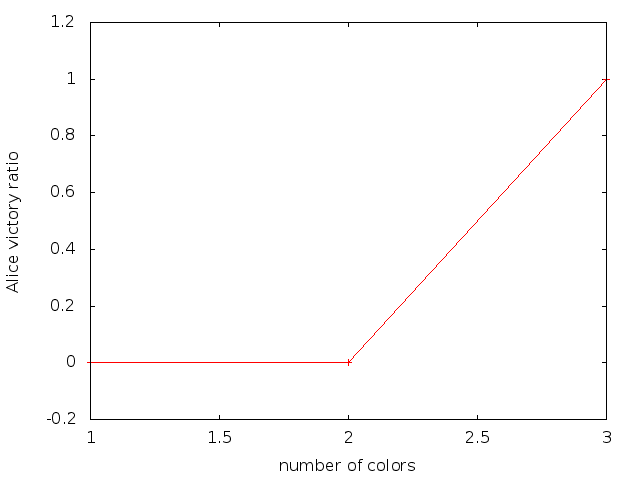
\includegraphics[width=11cm]{resultats/cycleimpair.png}

\subsubsection{Even number of vertices}

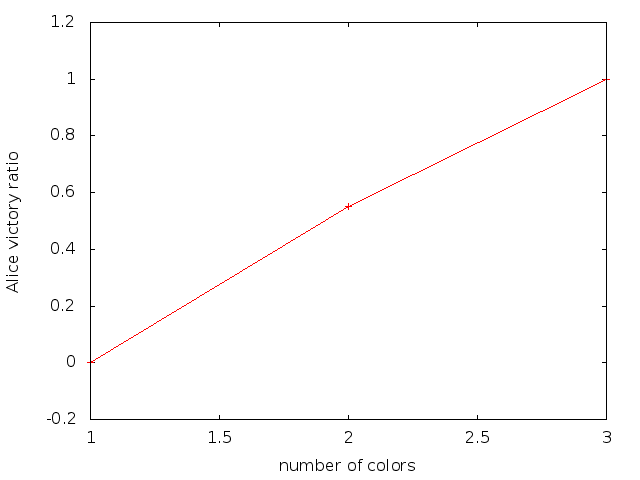
\includegraphics[width=11cm]{resultats/cyclepair.png}

\subsection{Grids}

\subsubsection{2x5}

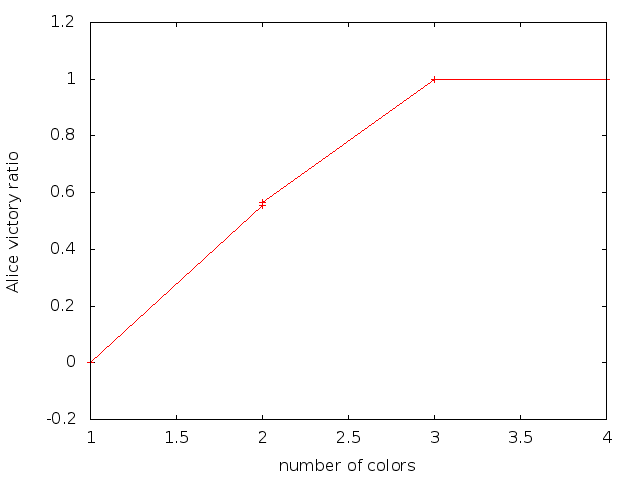
\includegraphics[width=11cm]{resultats/grille25.png}

\subsubsection{5x5}

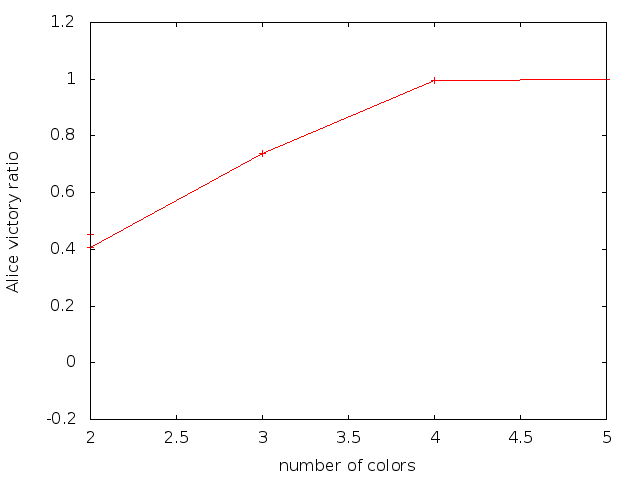
\includegraphics[width=11cm]{resultats/grille55.png}

\subsubsection{5x5 toroidal}

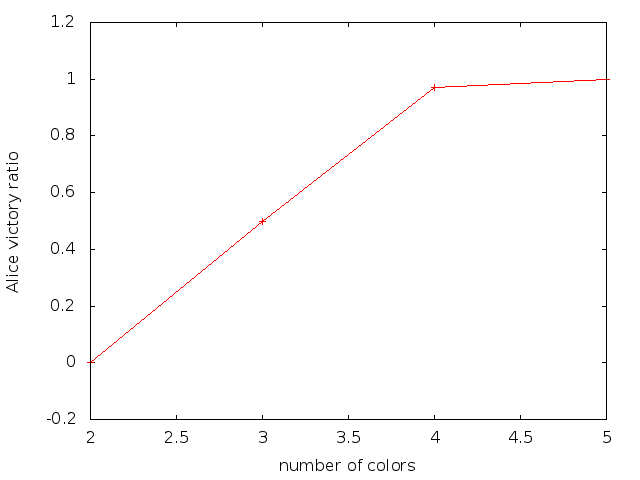
\includegraphics[width=11cm]{resultats/grilletor55.png}

\subsection{Binary Tree}

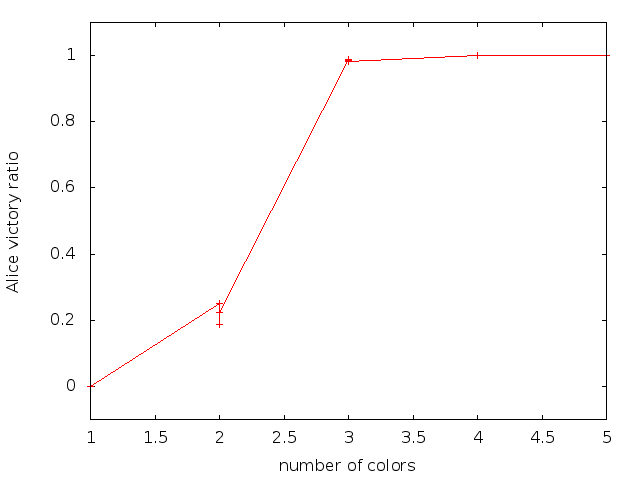
\includegraphics[width=11cm]{resultats/bintree3h.png}

\subsection{Non-Planar Graphs}

\subsubsection{Petersen Graph}

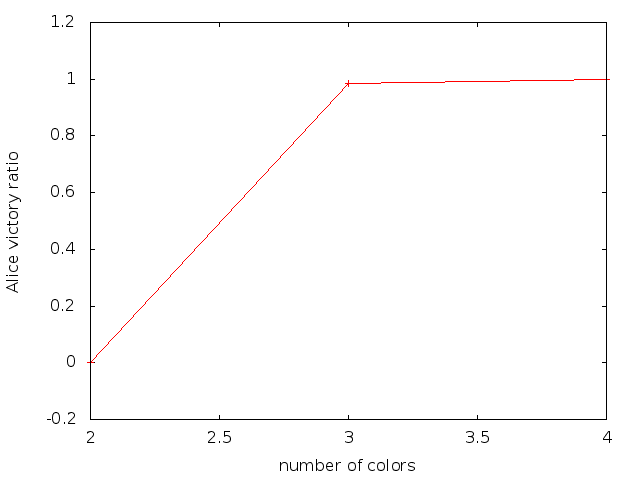
\includegraphics[width=11cm]{resultats/petersen.png}

\subsubsection{Icosaedron Graph}

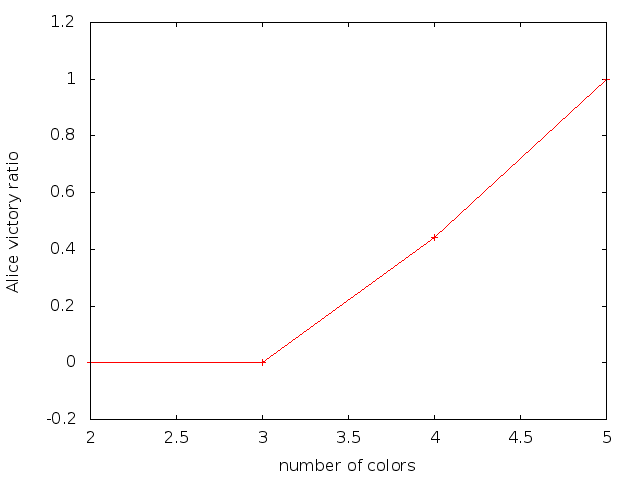
\includegraphics[width=11cm]{resultats/icosaedre.png}

\section{Results summary}

We recall that the game chromatic number of toroidal grids has been proved to be 5 in \cite{Raspaud20091183}. The Grotzsch graph was added later. We were therefore unable to calculate the theoretical values of each strategy in time.\\

\begin{tabular}{|l|c|c|c|c|c|}
\hline 
Graph & Chromatic number & Strategy 1 & Strategy 2 & Strategy 3 & Experimental results \\ 
\hline 
Chain (odd) & 2 & 6 & 6 & 5 & 3 \\ 
\hline 
Chain (even) & 2 & 6 & 6 & 5 & 3 \\ 
\hline 
Cycle (odd) & 3 & 12 & 12 & 8 & 3 \\ 
\hline 
Cycle (even) & 2 & 8 & 12 & 8 & 3 \\ 
\hline 
Grid 2x5 & 2 & 6 & 12 & 5 & 3 \\ 
\hline 
Grid 5x5 & 2 & 10 & 12 & 11 & 5 \\ 
\hline 
Grid 5x5 tor & 3 & 5 & 5 & 5 & 5 \\ 
\hline 
Binary tree & 2 & 6 & 6 & 5 & 4 \\ 
\hline 
Petersen & 3 & 18 & 12 & 14 & 4 \\ 
\hline 
Icosahedron & 4 & 32 & 20 & 20 & 5 \\ 
\hline 
Grotzsch & 4 & ? & ? & ? & 4 \\ 
\hline 
\end{tabular} 
\\
\\
We observe that the experimental values ​​are far below the theoretical values​​, especially regarding the Petersen graph and the icosahedron.

 %Expliquer les expériences réalisées, montrer en quoi elles sont pertinentes. Puis montrer quels objectifs ont été atteints. Caractériser le système (sur quoi notre logiciel marche bien, à partir de quand ça se dégrade etc.).
\chapter{Conclusion}
\minitoc

\section{Assessment}

Overall, we can say that the results are quite positive. Indeed, we were able to meet the original objectives and our results are better than what we expected.

We believe it is possible that there is a theoritical model which outperforms those presented in the article we studied.

\subsection{Experimental biases}

We have reason to believe that our protocols of experimentation can be improved to provide more reliable results:

\begin{itemize}
\item We can not make Alice or Bob stronger. If we increase the number of simulation performed by Alice, Bob will also increase the number of simulations that he performs, thus increasing its strength as much as that of Alice. Furthermore, the goal is to see whether Alice can win regardless of the strength of Bob, but our Bob is not infaillible.
\item Unlike the strategies of the article, our AI adapts itself based on the simulations it performs. Where a theoretical model always redo the same thing which seems to be the best choice, our AI adapts itself and will \textit{know} if a move leads to a victory or not, thus being able to out of an impasse.
\end{itemize}



\section{If we were to do it again...}


\section{Perspectives}




\appendix

\chapter{Diagrammes}

%\section{Architecture}\label{annexe-archi-initiale}


\chapter{Manuel de maintenance}

%\section{Conventions de codage}\label{annexe-conventions}

\subsection{Langue}

La langue du code doit impérativement être l'Anglais. Les variables, les objets, les classes et les méthodes sont nommés en Anglais.

Les commentaires doivent être écrit de préférence en Anglais. Néanmoins, le Français sera toléré (il vaut mieux écrire quelque chose de compréhensible en Français qu'un truc qui ne veut rien dire en Anglais).

La documentation, elle, est écrite en Français.

\subsection{Forme du code}

\subsubsection{Indentation}

L'indentation doit être effectuée à coup de \textbf{4 espaces}. Ne \textbf{pas} utiliser de tabulation dans le code !

\subsubsection{Opérateurs}

Les opérations utilisant des opérateurs doivent être espacées. De même pour les opérateurs de comparaisons…
Exemple : \verb!toto = tata + titi;! et non pas \verb!toto=tata+titi;! 

\subsubsection{Blocs}

Les blocs se présentent de la forme suivante (exemple avec un if) :
\begin{verbatim}
if (toto == tata) {
    tutu();
}
\end{verbatim}

\textbf{Aucune} autre forme de présentation n'est acceptée ! Pas de crochet ouvrant à la ligne, par exemple.

\begin{note}
  Les blocs if, for… contenant une seule instruction doivent \textbf{quand même} posséder des accolades. Ceci permet d'ajouter plus simplement des instructions si nécessaire, et le code n'en est que plus lisible, on voit bien la hiérarchie des blocs qui se ferment.
\end{note}

\subsubsection{Instructions ternaires}

Les instructions ternaires sont autorisées. En cas d'écriture complexe (plusieurs instructions imbriquées), un commentaire peut-être laissé en fin de ligne. 
Exemple : 
\begin{verbatim}
toto = (tata == 0)?1:10; // Si tata == 0, toto = 1, sinon, toto = 10
                         // mais ce commentaire n'est vraiment pas utile.
\end{verbatim}

\subsection{Contenu du code}

\subsubsection{Classes et Méthodes}

Afin de respecter les principes d'encapsulation, les attributs des classes doivent autant que possible être protected ou private. Pour y accéder, les classes proposent des accesseurs (setter et getter).

\subsubsection{Constructeurs et Destructeurs}

Toute classe doit posséder un destructeur, même s'il est vide.

\subsubsection{Magic Numbers}

Les « magic numbers » sont à éviter. Par exemple : \verb+if (toto == 4) { }+. D'où sort ce `4' ? C'est un « magic number ». Il vaudra donc mieux le remplacer par une constante globale, voire par un \#define, pour savoir à quoi il correspond et pouvoir paramétrer la classe simplement.
Exemple plus lisible :
\begin{verbatim}
#define MAX_THREADS 4
// blabla
if (toto == MAX_THREADS) { } 
\end{verbatim}

\begin{note}
Il peut bien sûr y avoir des exceptions. Les valeurs de 0 et de 1 sont parfaitement tolérées, par exemple.
\end{note}

\subsubsection{Mot clé const}

\begin{itemize}
  \item Si une méthode ne modifie pas l'objet lorsqu'elle est appelée, elle \textbf{doit} être déclarée \verb+const+.
  \item Si un argument d'une méthode n'est pas modifié dans la méthode, il \textbf{doit} être déclaré \verb+const+.
  \item Si un argument d'une méthode est succeptible d'être un gros objet, il devrait généralement être passé par référence constante, et non par copie (exemple : \verb+void setName(string const& name);+).
\end{itemize}

Ces règles permettent d'améliorer significativement la qualité du programme en fournissant des informations importantes au compilateur, mais aussi aux développeurs.

\subsection{Nomage}

Les noms sont tous donnés en anglais, donc la phrase qui suit ne devrait pas être précisée, mais on ne sait jamais… 
\textbf{Jamais}, sous \textbf{aucun} prétexte, d'accent dans le code !

Les variables, objets, classes, fonctions, méthodes… sont nommées de la manière suivante :

\begin{itemize}
  \item \verb+ClassName+
  \item \verb+methodName+
  \item \verb+objectName+ ou \verb+objectname+ (suivant le cas, par exemple, filename est plus joli que fileName).
  \item \verb+CONSTANT_NAME+
  \item \verb+setAttribute+
  \item \verb+getAttribute+
  \item \verb+isAttributed+ (exemple : si l'attribut "enable" est un booléen, \verb+isEnabled()+)
\end{itemize}

\subsubsection{Fichiers}

Les fichiers sont nommés en minuscules, sans espace ni underscore, et se terminent par .h, .cpp.

Par exemple, la classe \verb+ClassName+ sera donc contenue dans les fichiers \verb+classname.h+ et \verb+classname.cpp+. 

\subsection{Commentaires}

Il y a deux types de commentaires.

\subsubsection{Doxygen}

Chaque classe, chaque méthode et chaque slot doivent être documentés à l'aide de Doxygen. 

\subsubsection{Gotcha Keywords}

Le code doit, à chaque fois que c'est nécessaire, contenir des « Gotcha Keywords ». Ces commentaires sont de la forme :
\begin{verbatim}
// :KEYWORD:pseudo:date: commentaire
// Suite du commentaire, si nécessaire
\end{verbatim}

\begin{description}
  \item[KEYWORD] peut être un mot clé dans la liste suivante : DOC, TRICKY, COMMENT, TODO, KLUDGE, WARNING, DEBUG, BUG, DEBUG
  \item[pseudo] est le pseudo de l'utilisateur qui pose le commentaire
  \item[date] \textbf{doit impérativement} être écrite de la forme YYMMDD. Par exemple, pour le 31 février 2012, la date sera 120231
\end{description}

Exemple de gotcha : 
\begin{verbatim}
// :TODO:cbadiola:130115: We must send the report! If we don't, we will get punished!
\end{verbatim}

Un script python\footnote{\url{http://git.meowstars.org/cgit.cgi/gotcha}} permet de sortir la synthèse des GOTCHA de tout un répertoire, très pratique lors de la phase de développement pour avoir une vision globale. N'hésitez donc pas à user et abuser de ce type de commentaires, et choisissant autant que possible le bon mot clé. 


\chapter{Extraits de code}

%\input{sections/annexe_bidule}


\backmatter

\nocite{*}
\bibliographystyle{plain-fr}
\bibliography{../refs.bib}

\listoffigures

\listoftables

%\tableofcontents

\newpage
\pagestyle{empty}

Rapport de projet d'études et de recherche.\\
The map coloring game.\\
Master 2, 2012

\vfill

Les sources de ce rapport sont disponibles librement sur %\url{http://}.

\bigskip

%Certaines images illustrant ce document sont extraites de nomdusite (\url{http://}). Elles sont disponibles sous licence Creative Commons ou dans le domaine public.

\end{document}
